% Created by tikzDevice version 0.10.1 on 2016-09-01 14:29:08
% !TEX encoding = UTF-8 Unicode
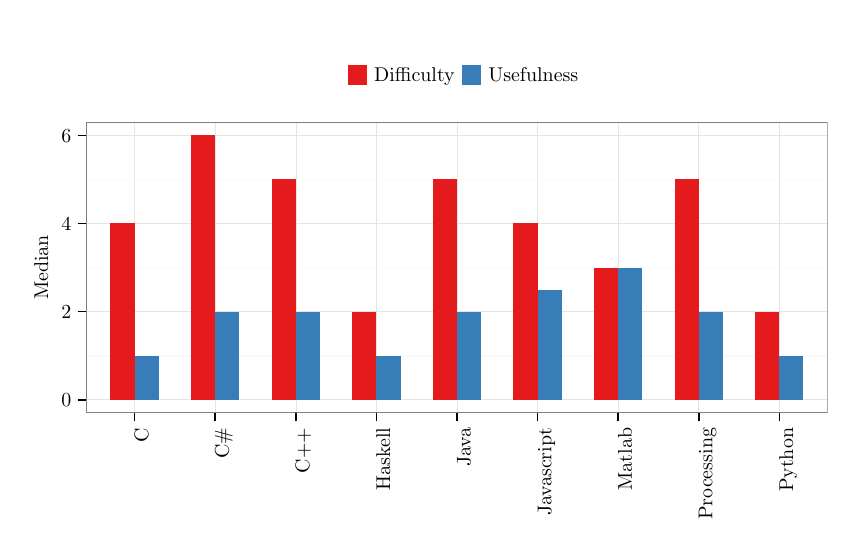
\begin{tikzpicture}[x=1pt,y=1pt]
\definecolor{fillColor}{RGB}{255,255,255}
\path[use as bounding box,fill=fillColor,fill opacity=0.00] (0,0) rectangle (289.08,180.67);
\begin{scope}
\path[clip] (  0.00,  0.00) rectangle (289.08,180.67);
\definecolor{drawColor}{RGB}{255,255,255}
\definecolor{fillColor}{RGB}{255,255,255}

\path[draw=drawColor,line width= 0.6pt,line join=round,line cap=round,fill=fillColor] (  0.00,  0.00) rectangle (289.08,180.67);
\end{scope}
\begin{scope}
\path[clip] ( 21.16, 41.44) rectangle (289.08,146.53);
\definecolor{fillColor}{RGB}{255,255,255}

\path[fill=fillColor] ( 21.16, 41.44) rectangle (289.08,146.53);
\definecolor{drawColor}{gray}{0.98}

\path[draw=drawColor,line width= 0.6pt,line join=round] ( 21.16, 62.14) --
	(289.08, 62.14);

\path[draw=drawColor,line width= 0.6pt,line join=round] ( 21.16, 93.98) --
	(289.08, 93.98);

\path[draw=drawColor,line width= 0.6pt,line join=round] ( 21.16,125.83) --
	(289.08,125.83);
\definecolor{drawColor}{gray}{0.90}

\path[draw=drawColor,line width= 0.2pt,line join=round] ( 21.16, 46.21) --
	(289.08, 46.21);

\path[draw=drawColor,line width= 0.2pt,line join=round] ( 21.16, 78.06) --
	(289.08, 78.06);

\path[draw=drawColor,line width= 0.2pt,line join=round] ( 21.16,109.91) --
	(289.08,109.91);

\path[draw=drawColor,line width= 0.2pt,line join=round] ( 21.16,141.75) --
	(289.08,141.75);

\path[draw=drawColor,line width= 0.2pt,line join=round] ( 38.63, 41.44) --
	( 38.63,146.53);

\path[draw=drawColor,line width= 0.2pt,line join=round] ( 67.75, 41.44) --
	( 67.75,146.53);

\path[draw=drawColor,line width= 0.2pt,line join=round] ( 96.88, 41.44) --
	( 96.88,146.53);

\path[draw=drawColor,line width= 0.2pt,line join=round] (126.00, 41.44) --
	(126.00,146.53);

\path[draw=drawColor,line width= 0.2pt,line join=round] (155.12, 41.44) --
	(155.12,146.53);

\path[draw=drawColor,line width= 0.2pt,line join=round] (184.24, 41.44) --
	(184.24,146.53);

\path[draw=drawColor,line width= 0.2pt,line join=round] (213.36, 41.44) --
	(213.36,146.53);

\path[draw=drawColor,line width= 0.2pt,line join=round] (242.48, 41.44) --
	(242.48,146.53);

\path[draw=drawColor,line width= 0.2pt,line join=round] (271.61, 41.44) --
	(271.61,146.53);
\definecolor{fillColor}{RGB}{55,126,184}

\path[fill=fillColor] ( 38.63, 46.21) rectangle ( 47.37, 62.14);
\definecolor{fillColor}{RGB}{228,26,28}

\path[fill=fillColor] ( 29.89, 46.21) rectangle ( 38.63,109.91);
\definecolor{fillColor}{RGB}{55,126,184}

\path[fill=fillColor] ( 67.75, 46.21) rectangle ( 76.49, 78.06);
\definecolor{fillColor}{RGB}{228,26,28}

\path[fill=fillColor] ( 59.02, 46.21) rectangle ( 67.75,141.75);
\definecolor{fillColor}{RGB}{55,126,184}

\path[fill=fillColor] ( 96.88, 46.21) rectangle (105.61, 78.06);
\definecolor{fillColor}{RGB}{228,26,28}

\path[fill=fillColor] ( 88.14, 46.21) rectangle ( 96.88,125.83);
\definecolor{fillColor}{RGB}{55,126,184}

\path[fill=fillColor] (126.00, 46.21) rectangle (134.73, 62.14);
\definecolor{fillColor}{RGB}{228,26,28}

\path[fill=fillColor] (117.26, 46.21) rectangle (126.00, 78.06);
\definecolor{fillColor}{RGB}{55,126,184}

\path[fill=fillColor] (155.12, 46.21) rectangle (163.86, 78.06);
\definecolor{fillColor}{RGB}{228,26,28}

\path[fill=fillColor] (146.38, 46.21) rectangle (155.12,125.83);
\definecolor{fillColor}{RGB}{55,126,184}

\path[fill=fillColor] (184.24, 46.21) rectangle (192.98, 86.02);
\definecolor{fillColor}{RGB}{228,26,28}

\path[fill=fillColor] (175.50, 46.21) rectangle (184.24,109.91);
\definecolor{fillColor}{RGB}{55,126,184}

\path[fill=fillColor] (213.36, 46.21) rectangle (222.10, 93.98);
\definecolor{fillColor}{RGB}{228,26,28}

\path[fill=fillColor] (204.63, 46.21) rectangle (213.36, 93.98);
\definecolor{fillColor}{RGB}{55,126,184}

\path[fill=fillColor] (242.48, 46.21) rectangle (251.22, 78.06);
\definecolor{fillColor}{RGB}{228,26,28}

\path[fill=fillColor] (233.75, 46.21) rectangle (242.48,125.83);
\definecolor{fillColor}{RGB}{55,126,184}

\path[fill=fillColor] (271.61, 46.21) rectangle (280.34, 62.14);
\definecolor{fillColor}{RGB}{228,26,28}

\path[fill=fillColor] (262.87, 46.21) rectangle (271.61, 78.06);
\definecolor{drawColor}{gray}{0.50}

\path[draw=drawColor,line width= 0.6pt,line join=round,line cap=round] ( 21.16, 41.44) rectangle (289.08,146.53);
\end{scope}
\begin{scope}
\path[clip] (  0.00,  0.00) rectangle (289.08,180.67);
\definecolor{drawColor}{RGB}{0,0,0}

\node[text=drawColor,anchor=base east,inner sep=0pt, outer sep=0pt, scale=  0.72] at ( 15.76, 43.73) {0};

\node[text=drawColor,anchor=base east,inner sep=0pt, outer sep=0pt, scale=  0.72] at ( 15.76, 75.58) {2};

\node[text=drawColor,anchor=base east,inner sep=0pt, outer sep=0pt, scale=  0.72] at ( 15.76,107.43) {4};

\node[text=drawColor,anchor=base east,inner sep=0pt, outer sep=0pt, scale=  0.72] at ( 15.76,139.28) {6};
\end{scope}
\begin{scope}
\path[clip] (  0.00,  0.00) rectangle (289.08,180.67);
\definecolor{drawColor}{RGB}{0,0,0}

\path[draw=drawColor,line width= 0.6pt,line join=round] ( 18.16, 46.21) --
	( 21.16, 46.21);

\path[draw=drawColor,line width= 0.6pt,line join=round] ( 18.16, 78.06) --
	( 21.16, 78.06);

\path[draw=drawColor,line width= 0.6pt,line join=round] ( 18.16,109.91) --
	( 21.16,109.91);

\path[draw=drawColor,line width= 0.6pt,line join=round] ( 18.16,141.75) --
	( 21.16,141.75);
\end{scope}
\begin{scope}
\path[clip] (  0.00,  0.00) rectangle (289.08,180.67);
\definecolor{drawColor}{RGB}{0,0,0}

\path[draw=drawColor,line width= 0.6pt,line join=round] ( 38.63, 38.44) --
	( 38.63, 41.44);

\path[draw=drawColor,line width= 0.6pt,line join=round] ( 67.75, 38.44) --
	( 67.75, 41.44);

\path[draw=drawColor,line width= 0.6pt,line join=round] ( 96.88, 38.44) --
	( 96.88, 41.44);

\path[draw=drawColor,line width= 0.6pt,line join=round] (126.00, 38.44) --
	(126.00, 41.44);

\path[draw=drawColor,line width= 0.6pt,line join=round] (155.12, 38.44) --
	(155.12, 41.44);

\path[draw=drawColor,line width= 0.6pt,line join=round] (184.24, 38.44) --
	(184.24, 41.44);

\path[draw=drawColor,line width= 0.6pt,line join=round] (213.36, 38.44) --
	(213.36, 41.44);

\path[draw=drawColor,line width= 0.6pt,line join=round] (242.48, 38.44) --
	(242.48, 41.44);

\path[draw=drawColor,line width= 0.6pt,line join=round] (271.61, 38.44) --
	(271.61, 41.44);
\end{scope}
\begin{scope}
\path[clip] (  0.00,  0.00) rectangle (289.08,180.67);
\definecolor{drawColor}{RGB}{0,0,0}

\node[text=drawColor,rotate= 90.00,anchor=base east,inner sep=0pt, outer sep=0pt, scale=  0.72] at ( 43.59, 36.04) {C};

\node[text=drawColor,rotate= 90.00,anchor=base east,inner sep=0pt, outer sep=0pt, scale=  0.72] at ( 72.71, 36.04) {C\#};

\node[text=drawColor,rotate= 90.00,anchor=base east,inner sep=0pt, outer sep=0pt, scale=  0.72] at (101.83, 36.04) {C++};

\node[text=drawColor,rotate= 90.00,anchor=base east,inner sep=0pt, outer sep=0pt, scale=  0.72] at (130.96, 36.04) {Haskell};

\node[text=drawColor,rotate= 90.00,anchor=base east,inner sep=0pt, outer sep=0pt, scale=  0.72] at (160.08, 36.04) {Java};

\node[text=drawColor,rotate= 90.00,anchor=base east,inner sep=0pt, outer sep=0pt, scale=  0.72] at (189.20, 36.04) {Javascript};

\node[text=drawColor,rotate= 90.00,anchor=base east,inner sep=0pt, outer sep=0pt, scale=  0.72] at (218.32, 36.04) {Matlab};

\node[text=drawColor,rotate= 90.00,anchor=base east,inner sep=0pt, outer sep=0pt, scale=  0.72] at (247.44, 36.04) {Processing};

\node[text=drawColor,rotate= 90.00,anchor=base east,inner sep=0pt, outer sep=0pt, scale=  0.72] at (276.57, 36.04) {Python};
\end{scope}
\begin{scope}
\path[clip] (  0.00,  0.00) rectangle (289.08,180.67);
\definecolor{drawColor}{RGB}{0,0,0}

\node[text=drawColor,rotate= 90.00,anchor=base,inner sep=0pt, outer sep=0pt, scale=  0.72] at (  7.36, 93.98) {Median};
\end{scope}
\begin{scope}
\path[clip] (  0.00,  0.00) rectangle (289.08,180.67);
\definecolor{fillColor}{RGB}{255,255,255}

\path[fill=fillColor] (107.00,155.07) rectangle (203.24,172.14);
\end{scope}
\begin{scope}
\path[clip] (  0.00,  0.00) rectangle (289.08,180.67);
\definecolor{fillColor}{RGB}{228,26,28}

\path[fill=fillColor] (115.59,160.05) rectangle (122.70,167.16);
\end{scope}
\begin{scope}
\path[clip] (  0.00,  0.00) rectangle (289.08,180.67);
\definecolor{fillColor}{RGB}{55,126,184}

\path[fill=fillColor] (156.83,160.05) rectangle (163.94,167.16);
\end{scope}
\begin{scope}
\path[clip] (  0.00,  0.00) rectangle (289.08,180.67);
\definecolor{drawColor}{RGB}{0,0,0}

\node[text=drawColor,anchor=base west,inner sep=0pt, outer sep=0pt, scale=  0.72] at (125.22,161.12) {Difficulty};
\end{scope}
\begin{scope}
\path[clip] (  0.00,  0.00) rectangle (289.08,180.67);
\definecolor{drawColor}{RGB}{0,0,0}

\node[text=drawColor,anchor=base west,inner sep=0pt, outer sep=0pt, scale=  0.72] at (166.46,161.12) {Usefulness};
\end{scope}
\end{tikzpicture}
